\section{Auswertung}
\label{sec:Auswertung}

Aus \autoref{tab:wertea} sind die Messwerte zu Aufgabenteil a) zu entnehmen.
\begin{table}[H]
    \centering
    \caption{Messwerte zur Wheatstone MessbrückeAufgabe a.}
    \label{tab:wertea}
    \begin{tabular}{c c}
    \toprule
    $U \:/\:$ V & $t \:/\:$ ms \\
    \midrule
    0,55 & 0,00 \\
    0,50 & 0,02 \\
    0,44 & 0,04 \\
    0,40 & 0,05 \\
    0,36 & 0,06 \\
    0,32 & 0,08 \\
    0,26 & 0,10 \\
    0,24 & 0,12 \\
    0,18 & 0,14 \\
    0,12 & 0,16 \\
    0,1 & 0,18 \\
    0,04 & 0,20 \\
    0,00 & 0,22 \\
    -0,04 & 0,24 \\
    -0,06 & 0,26 \\
    -0,10 & 0,28 \\
    -0,14 & 0,30 \\
    -0,16 & 0,32 \\
    -0,18 & 0,34 \\
    -0,22 & 0,36 \\
    -0,24 & 0,38 \\
    -0,28 & 0,40 \\
    -0,30 & 0,42 \\
    -0,32 & 0,44 \\
    -0,34 & 0,46 \\
    -0,38 & 0,48 \\
    -0,40 & 0,5 \\
    -0,42 & 0,52 \\
    -0,44 & 0,54 \\
    -0,46 & 0,56 \\
    -0,48 & 0,58 \\
    -0,50 & 0,6 \\
    \bottomrule
    \end{tabular}
\end{table}

Aus \autoref{fig:entladekurve} ist eine Abbildung der Entladekurve auf einem Oszilloskop zu entnehmen.
\begin{figure}
    \centering
    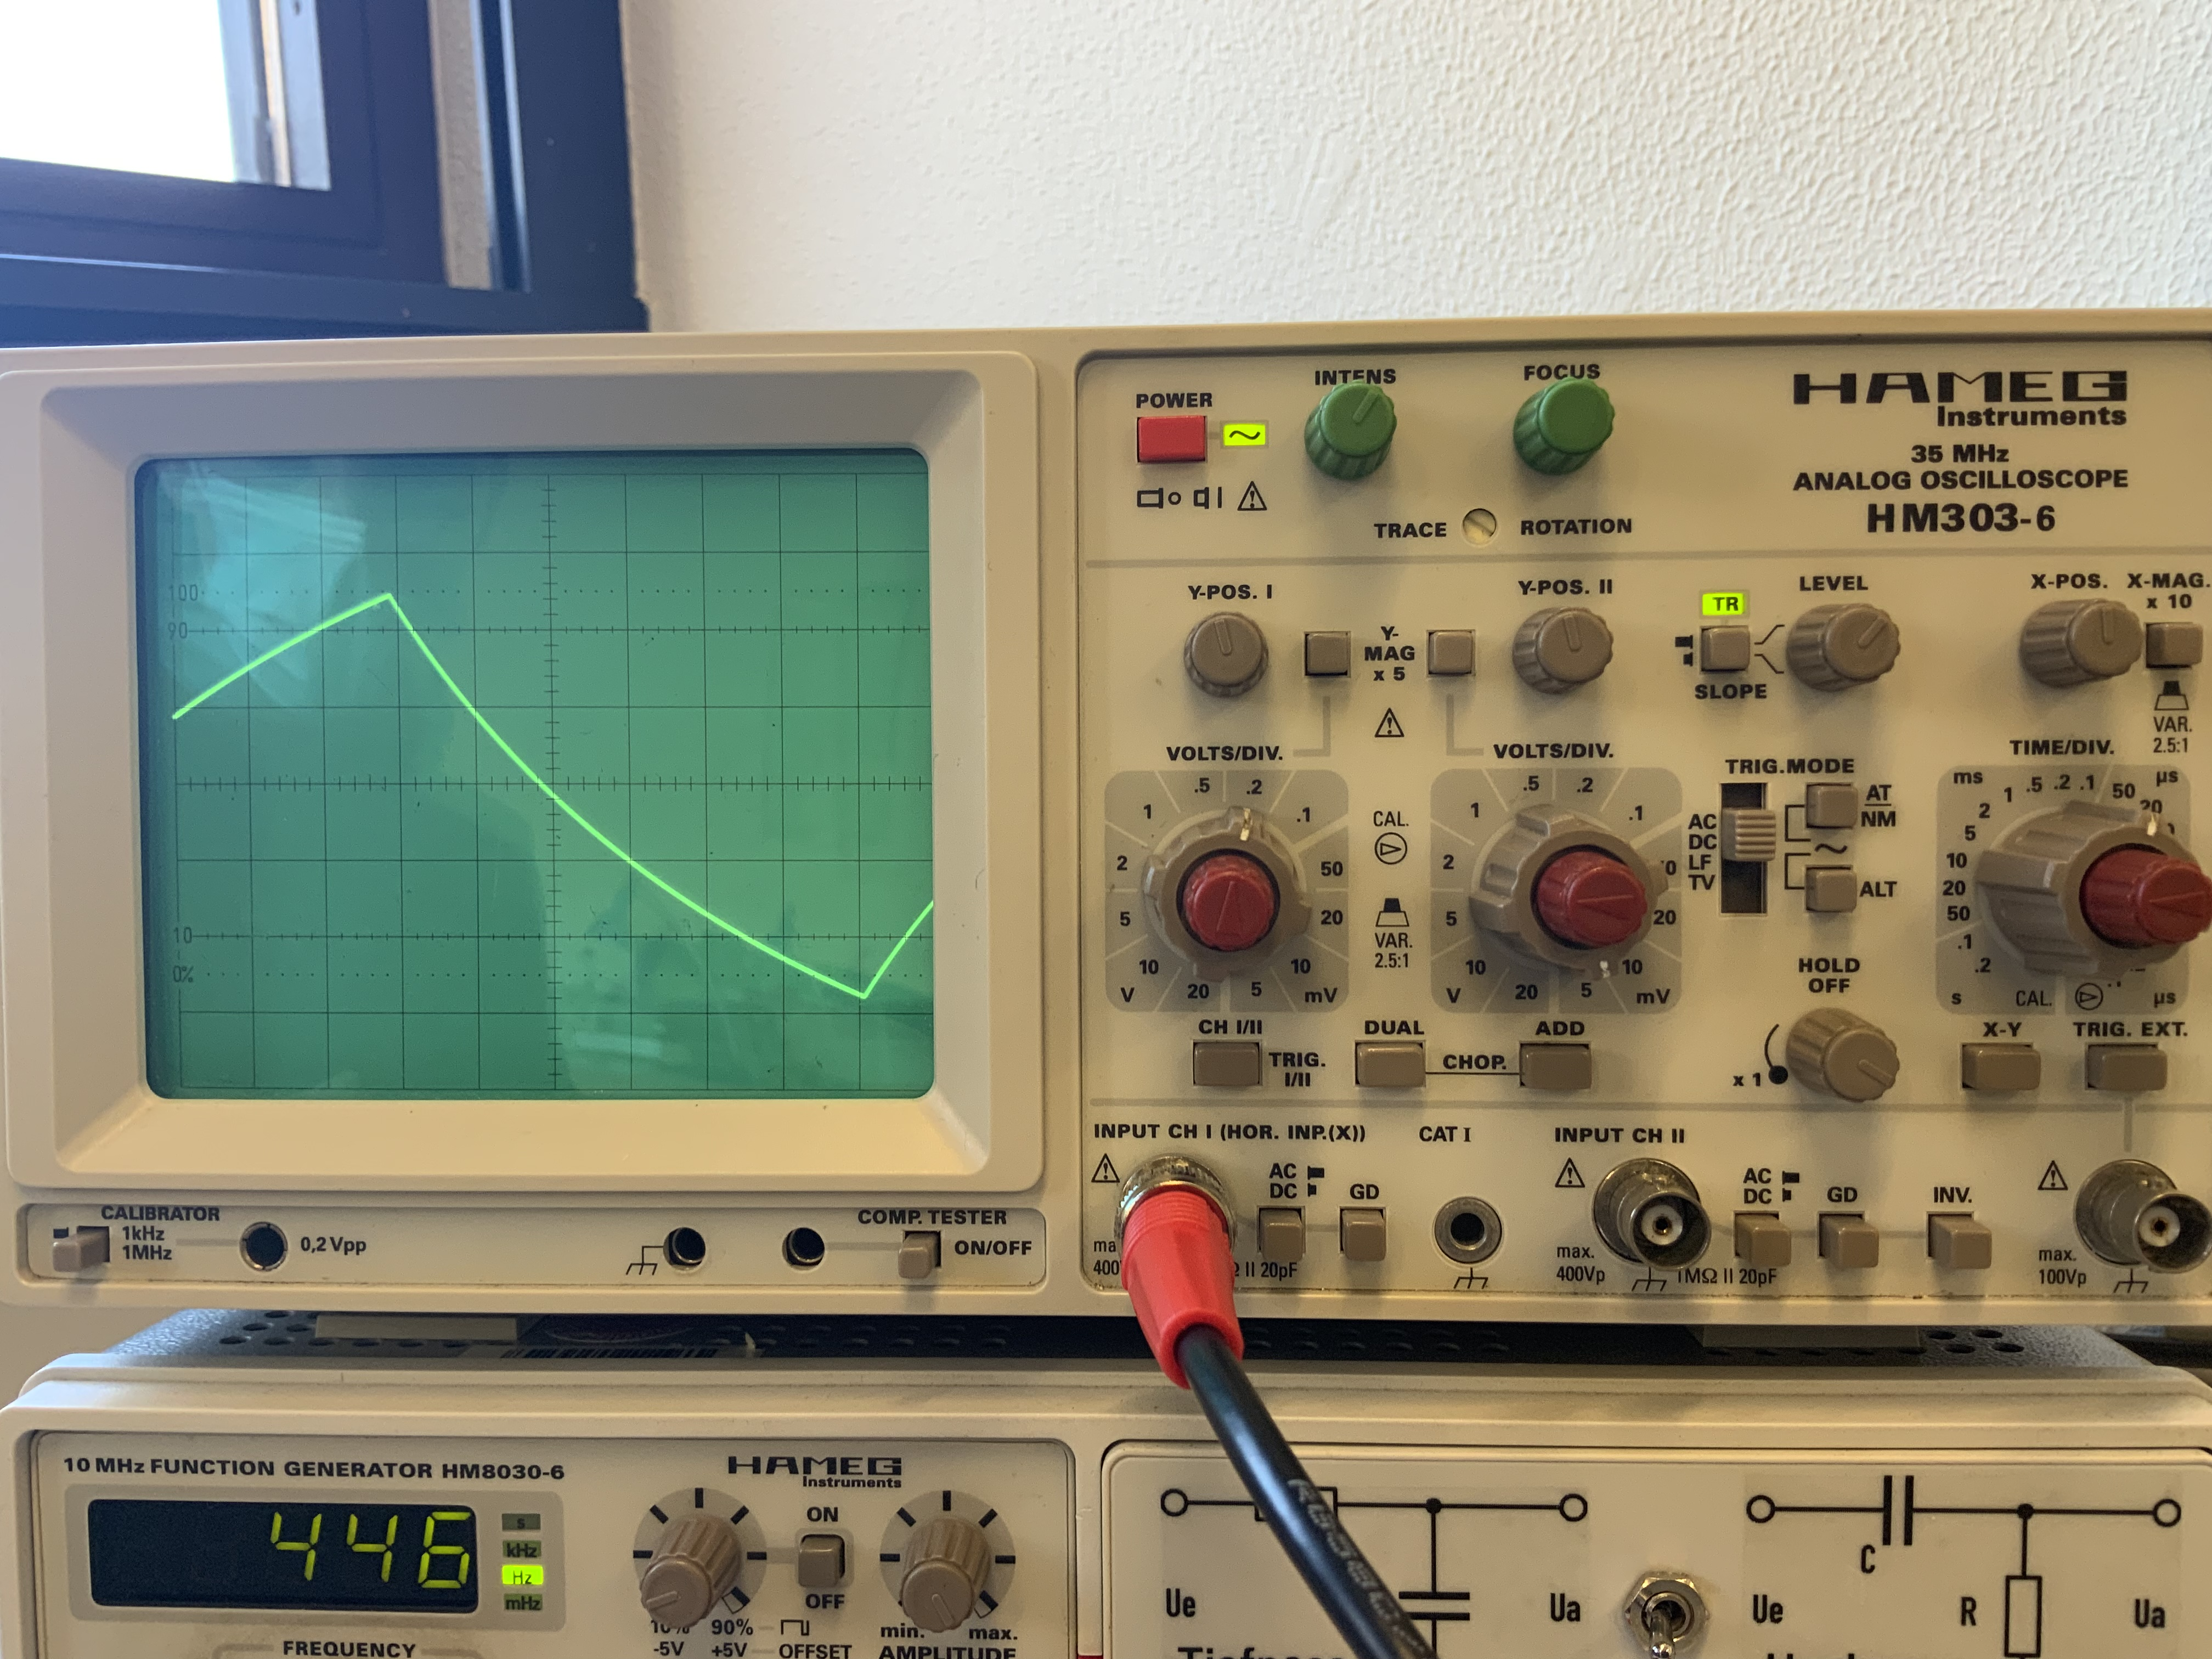
\includegraphics[width=0.75\textwidth]{Dateien/entladekurve.jpeg}
    \caption{Entladekurve.}
    \label{fig:entladekurve}
\end{figure}

Aus \autoref{fig:d.1}, \autoref{fig:d.2} und \autoref{fig:d.3} sind die Messwerte zu Aufgabenteil d) zu entnehmen.
\begin{figure}
    \centering
    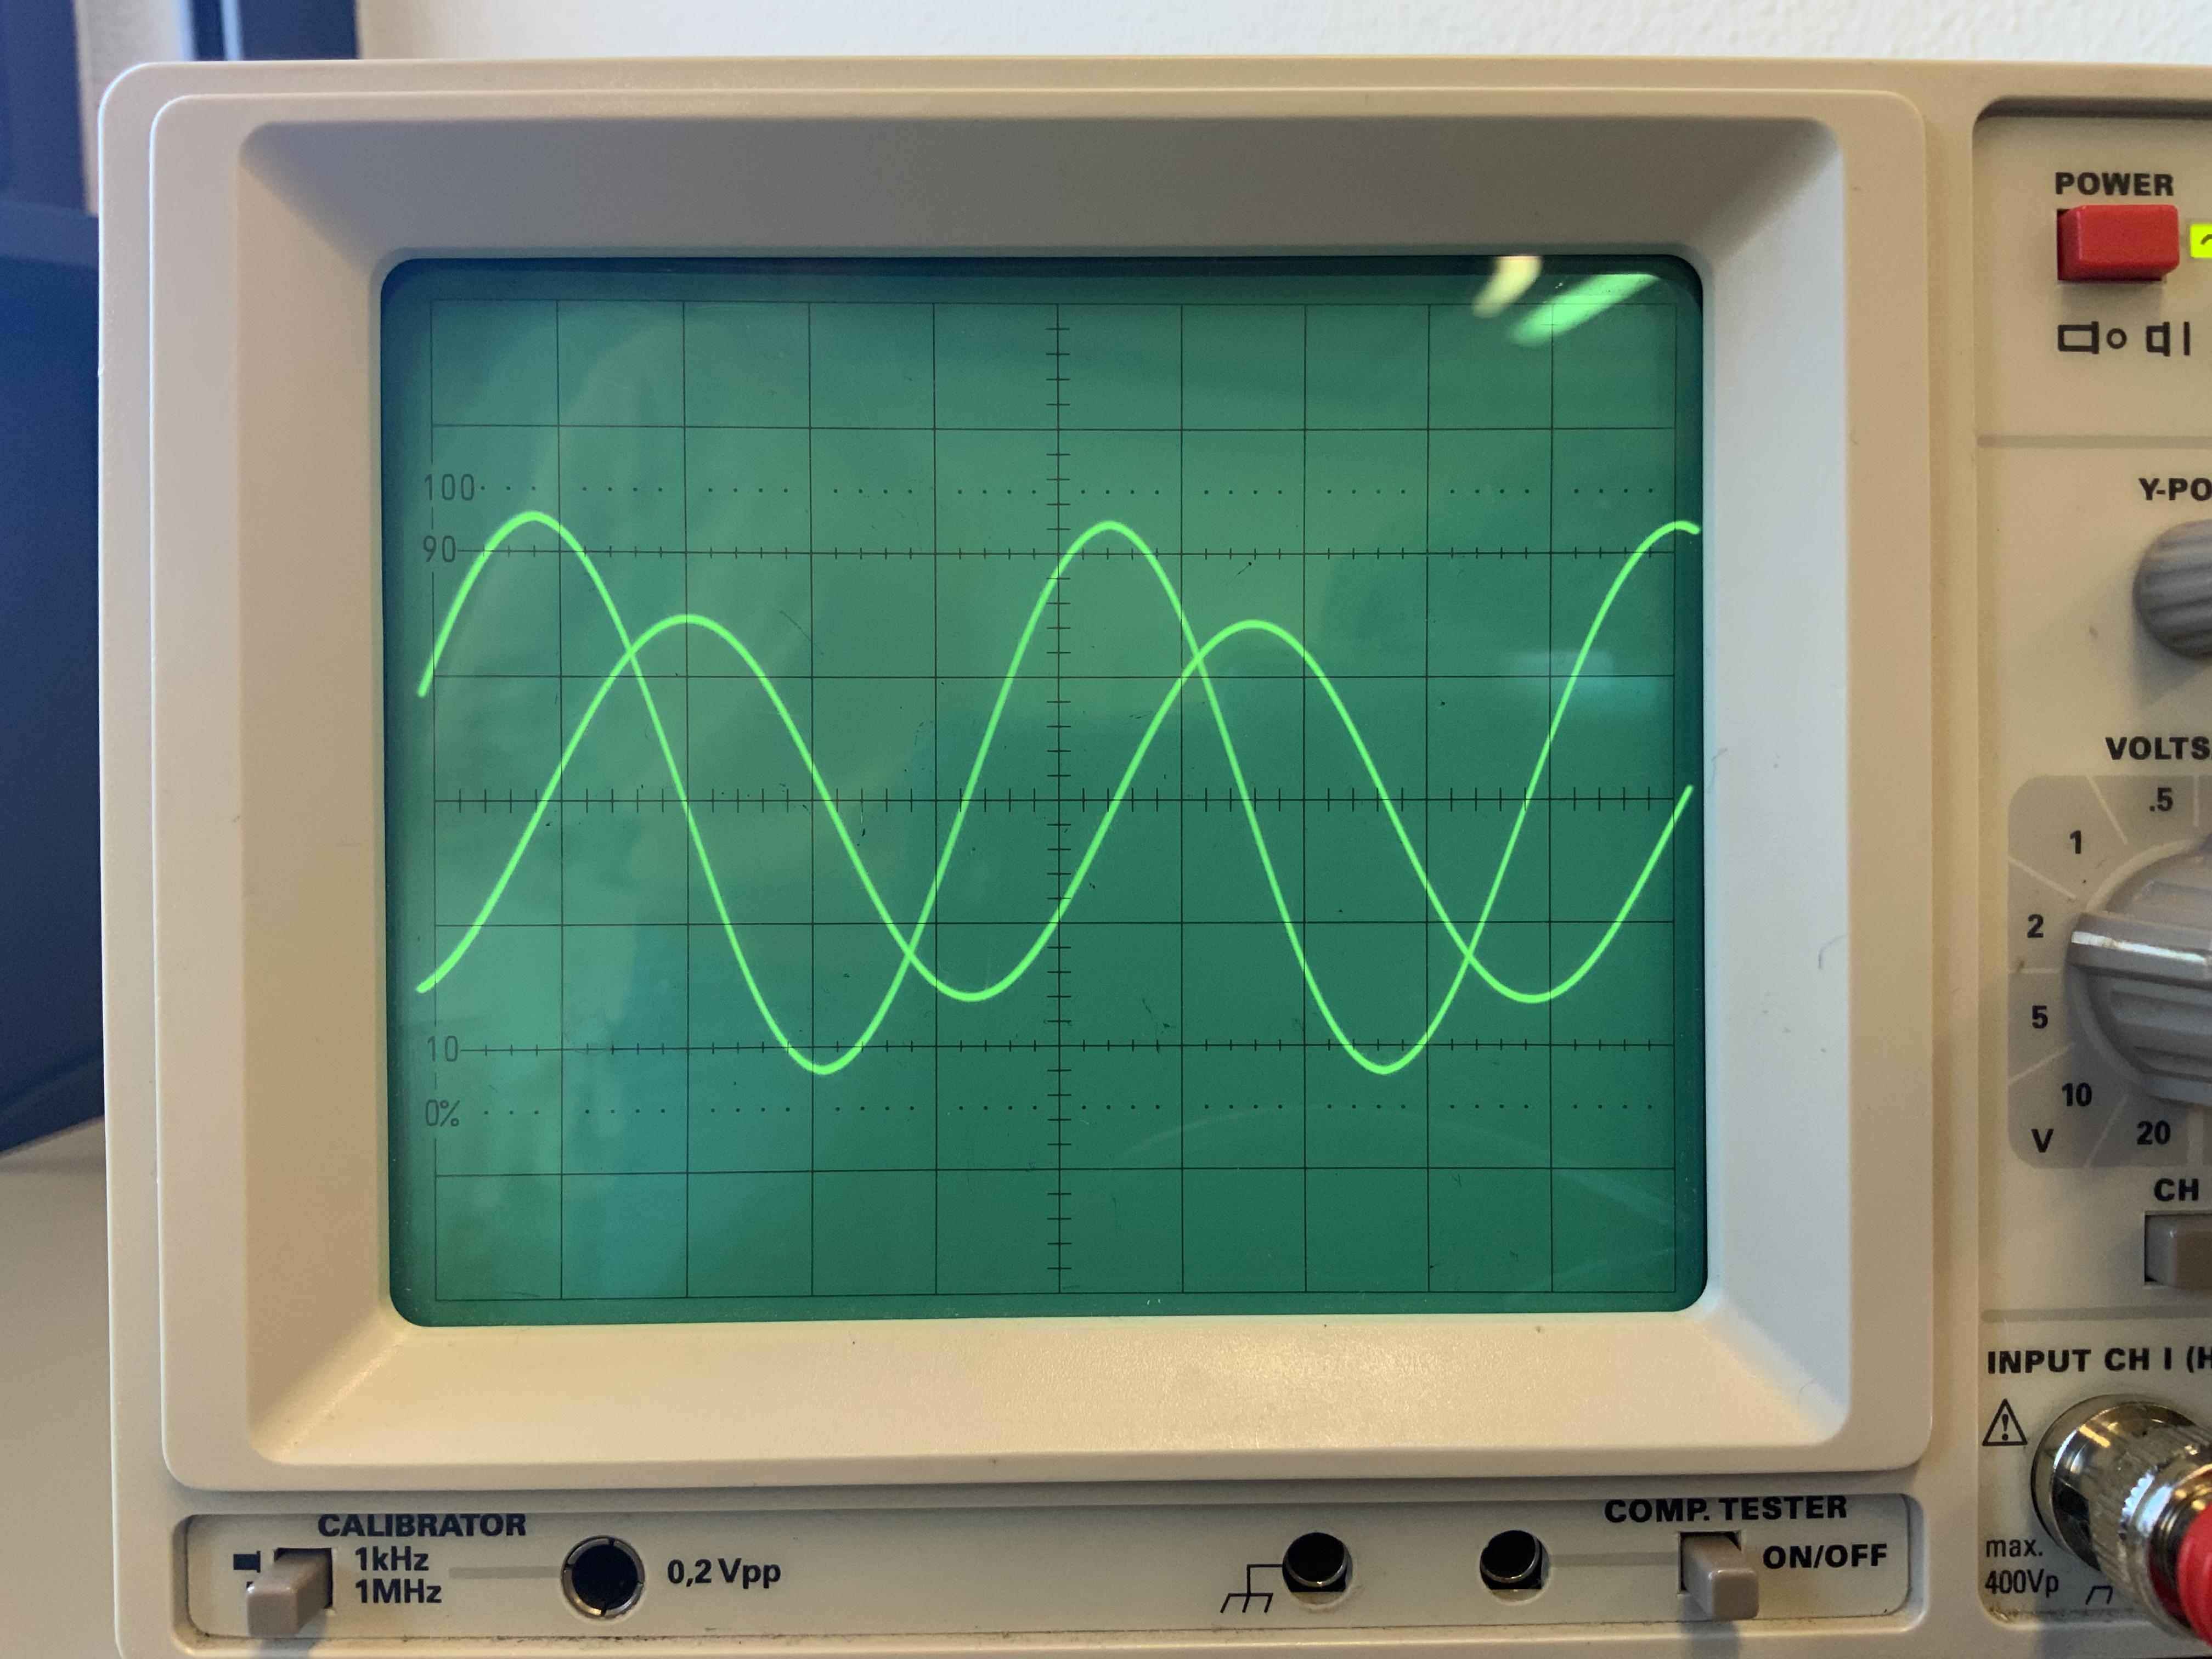
\includegraphics[width=0.75\textwidth]{Dateien/d.1.jpeg}
    \caption{Messdaten zu Aufgabenteil d).}
    \label{fig:d.1}
\end{figure}

\begin{figure}
    \centering
    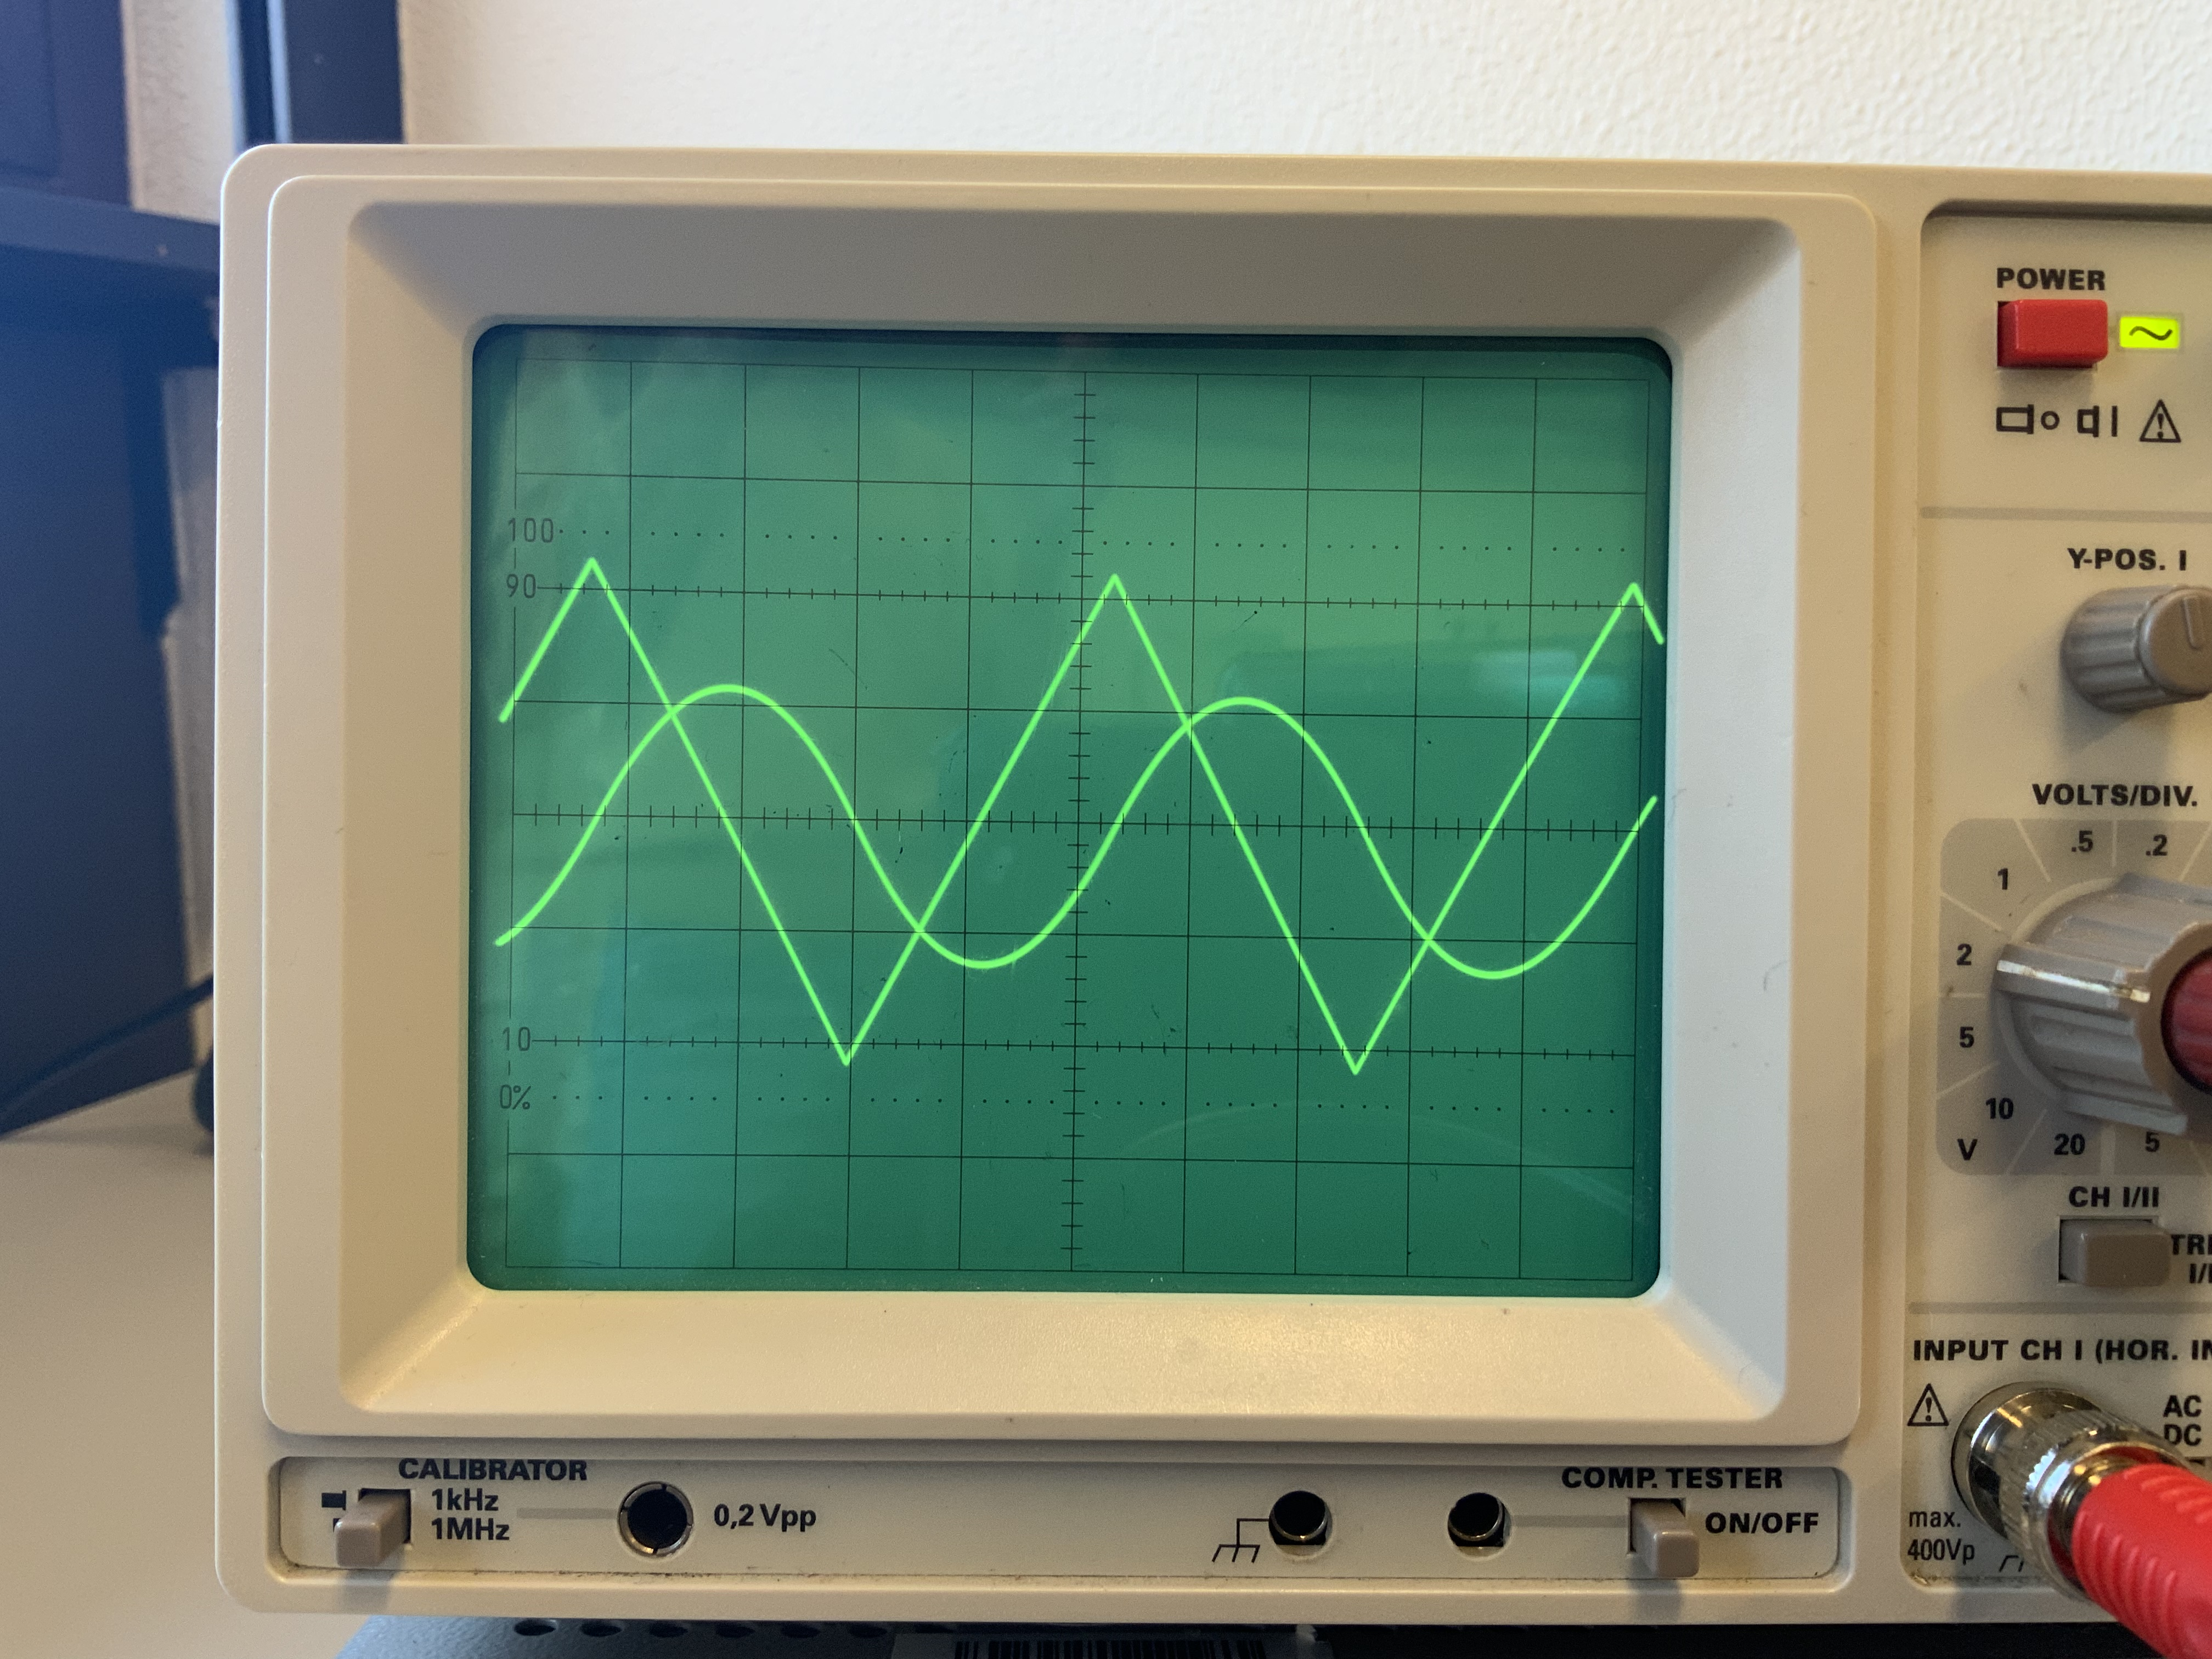
\includegraphics[width=0.75\textwidth]{Dateien/d.2.jpeg}
    \caption{Messdaten zu Aufgabenteil d).}
    \label{fig:d.2}
\end{figure}

\begin{figure}
    \centering
    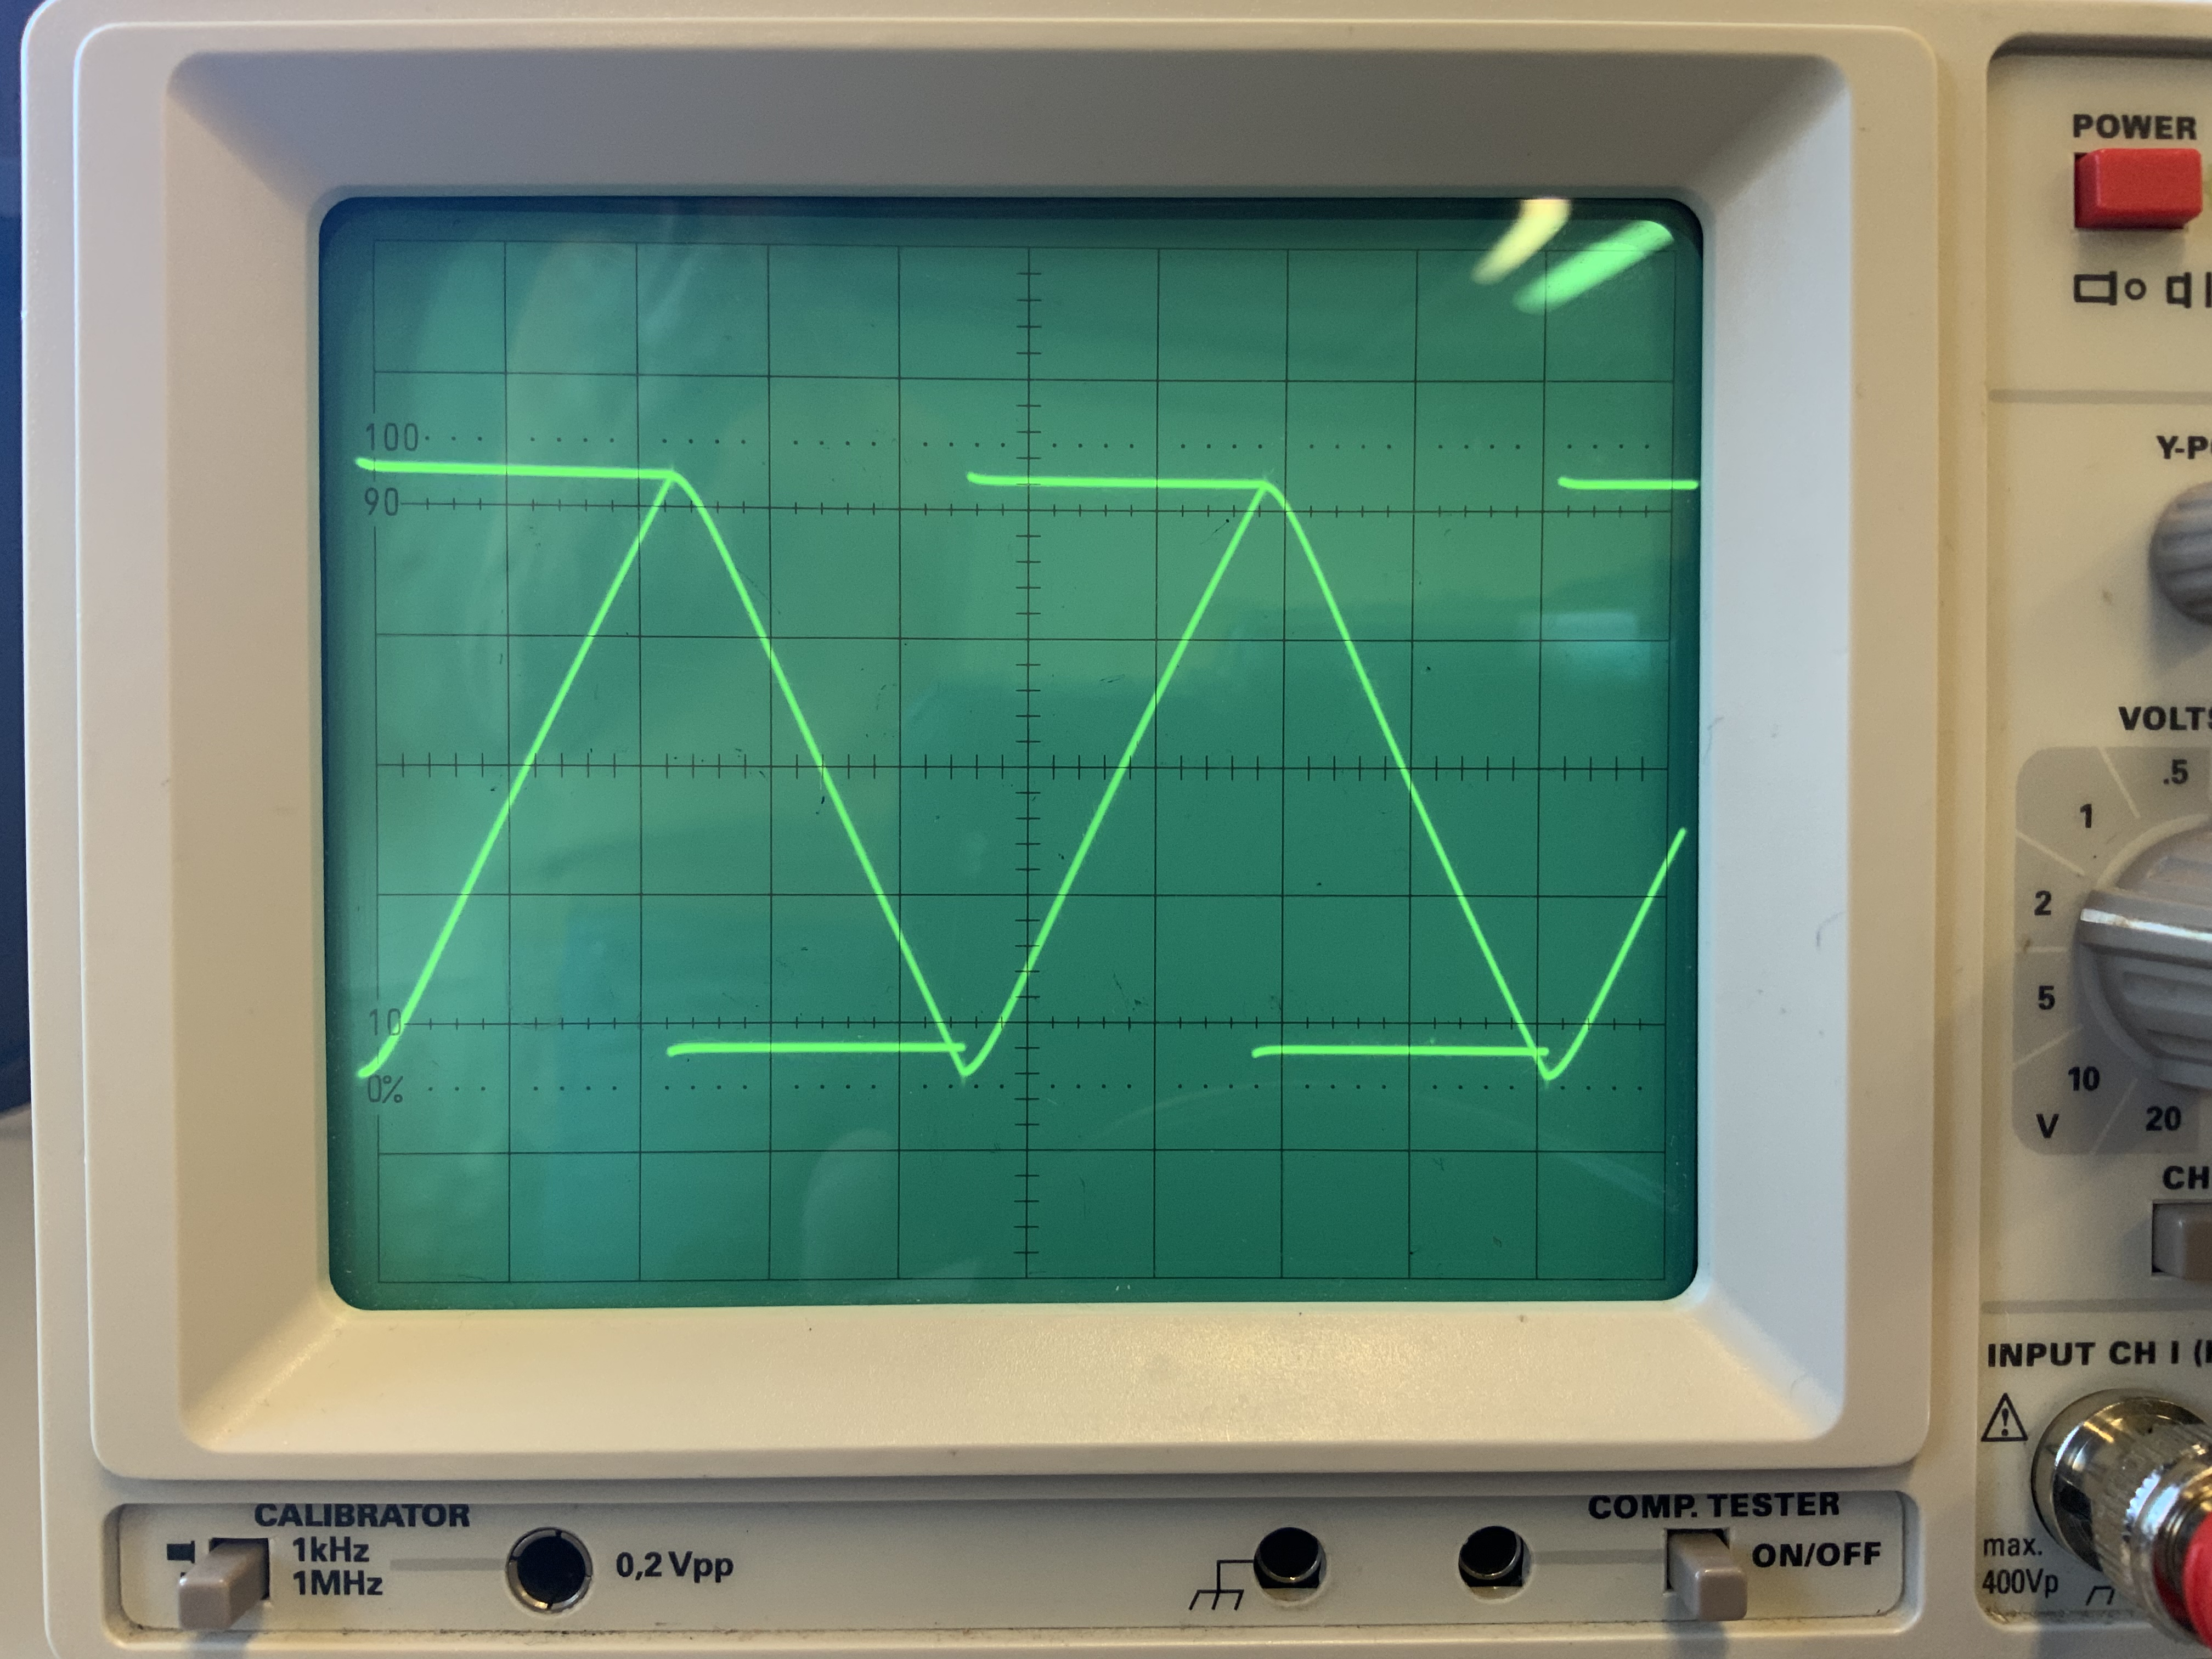
\includegraphics[width=0.75\textwidth]{Dateien/d.3.jpeg}
    \caption{Messdaten zu Aufgabenteil d).}
    \label{fig:d.3}
\end{figure}


%%%     Originale Messwerte
\begin{figure}
    \centering
    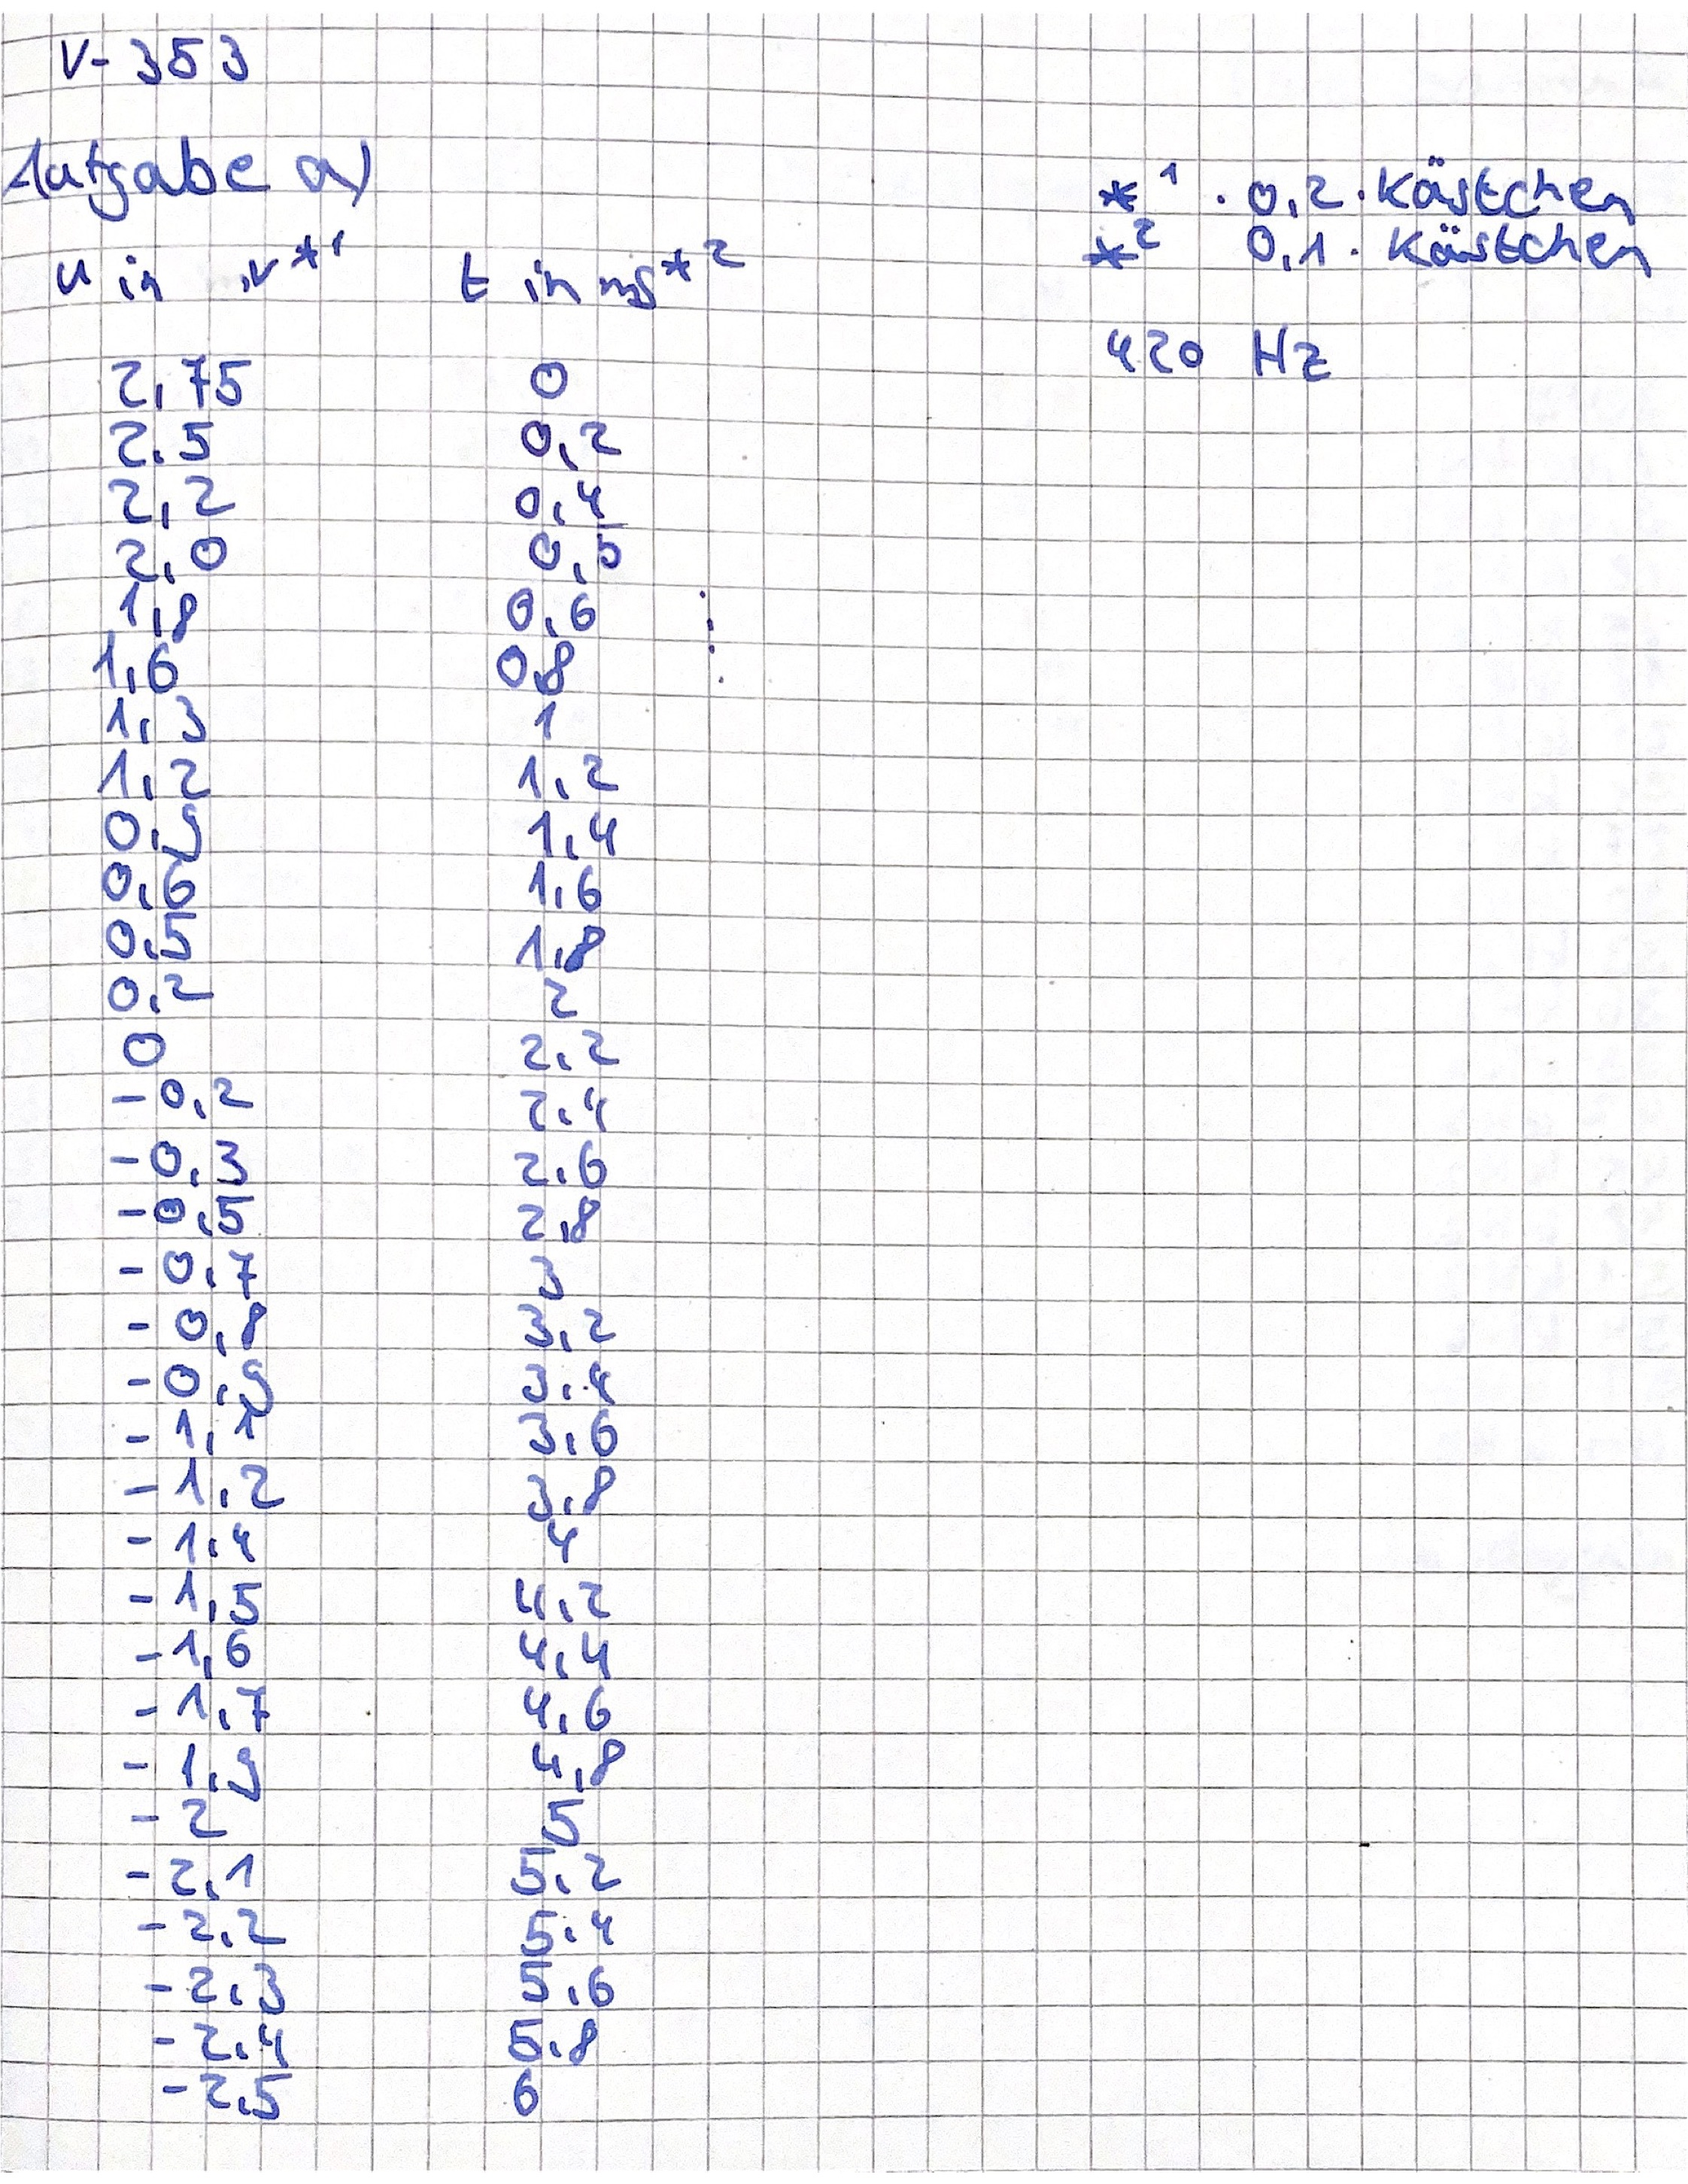
\includegraphics[width=0.75\textwidth]{Dateien/daten1.jpg}
    \caption{Originale Messdaten zu Aufgabenteil a).}
    \label{fig:daten1}
\end{figure}

\begin{figure}
    \centering
    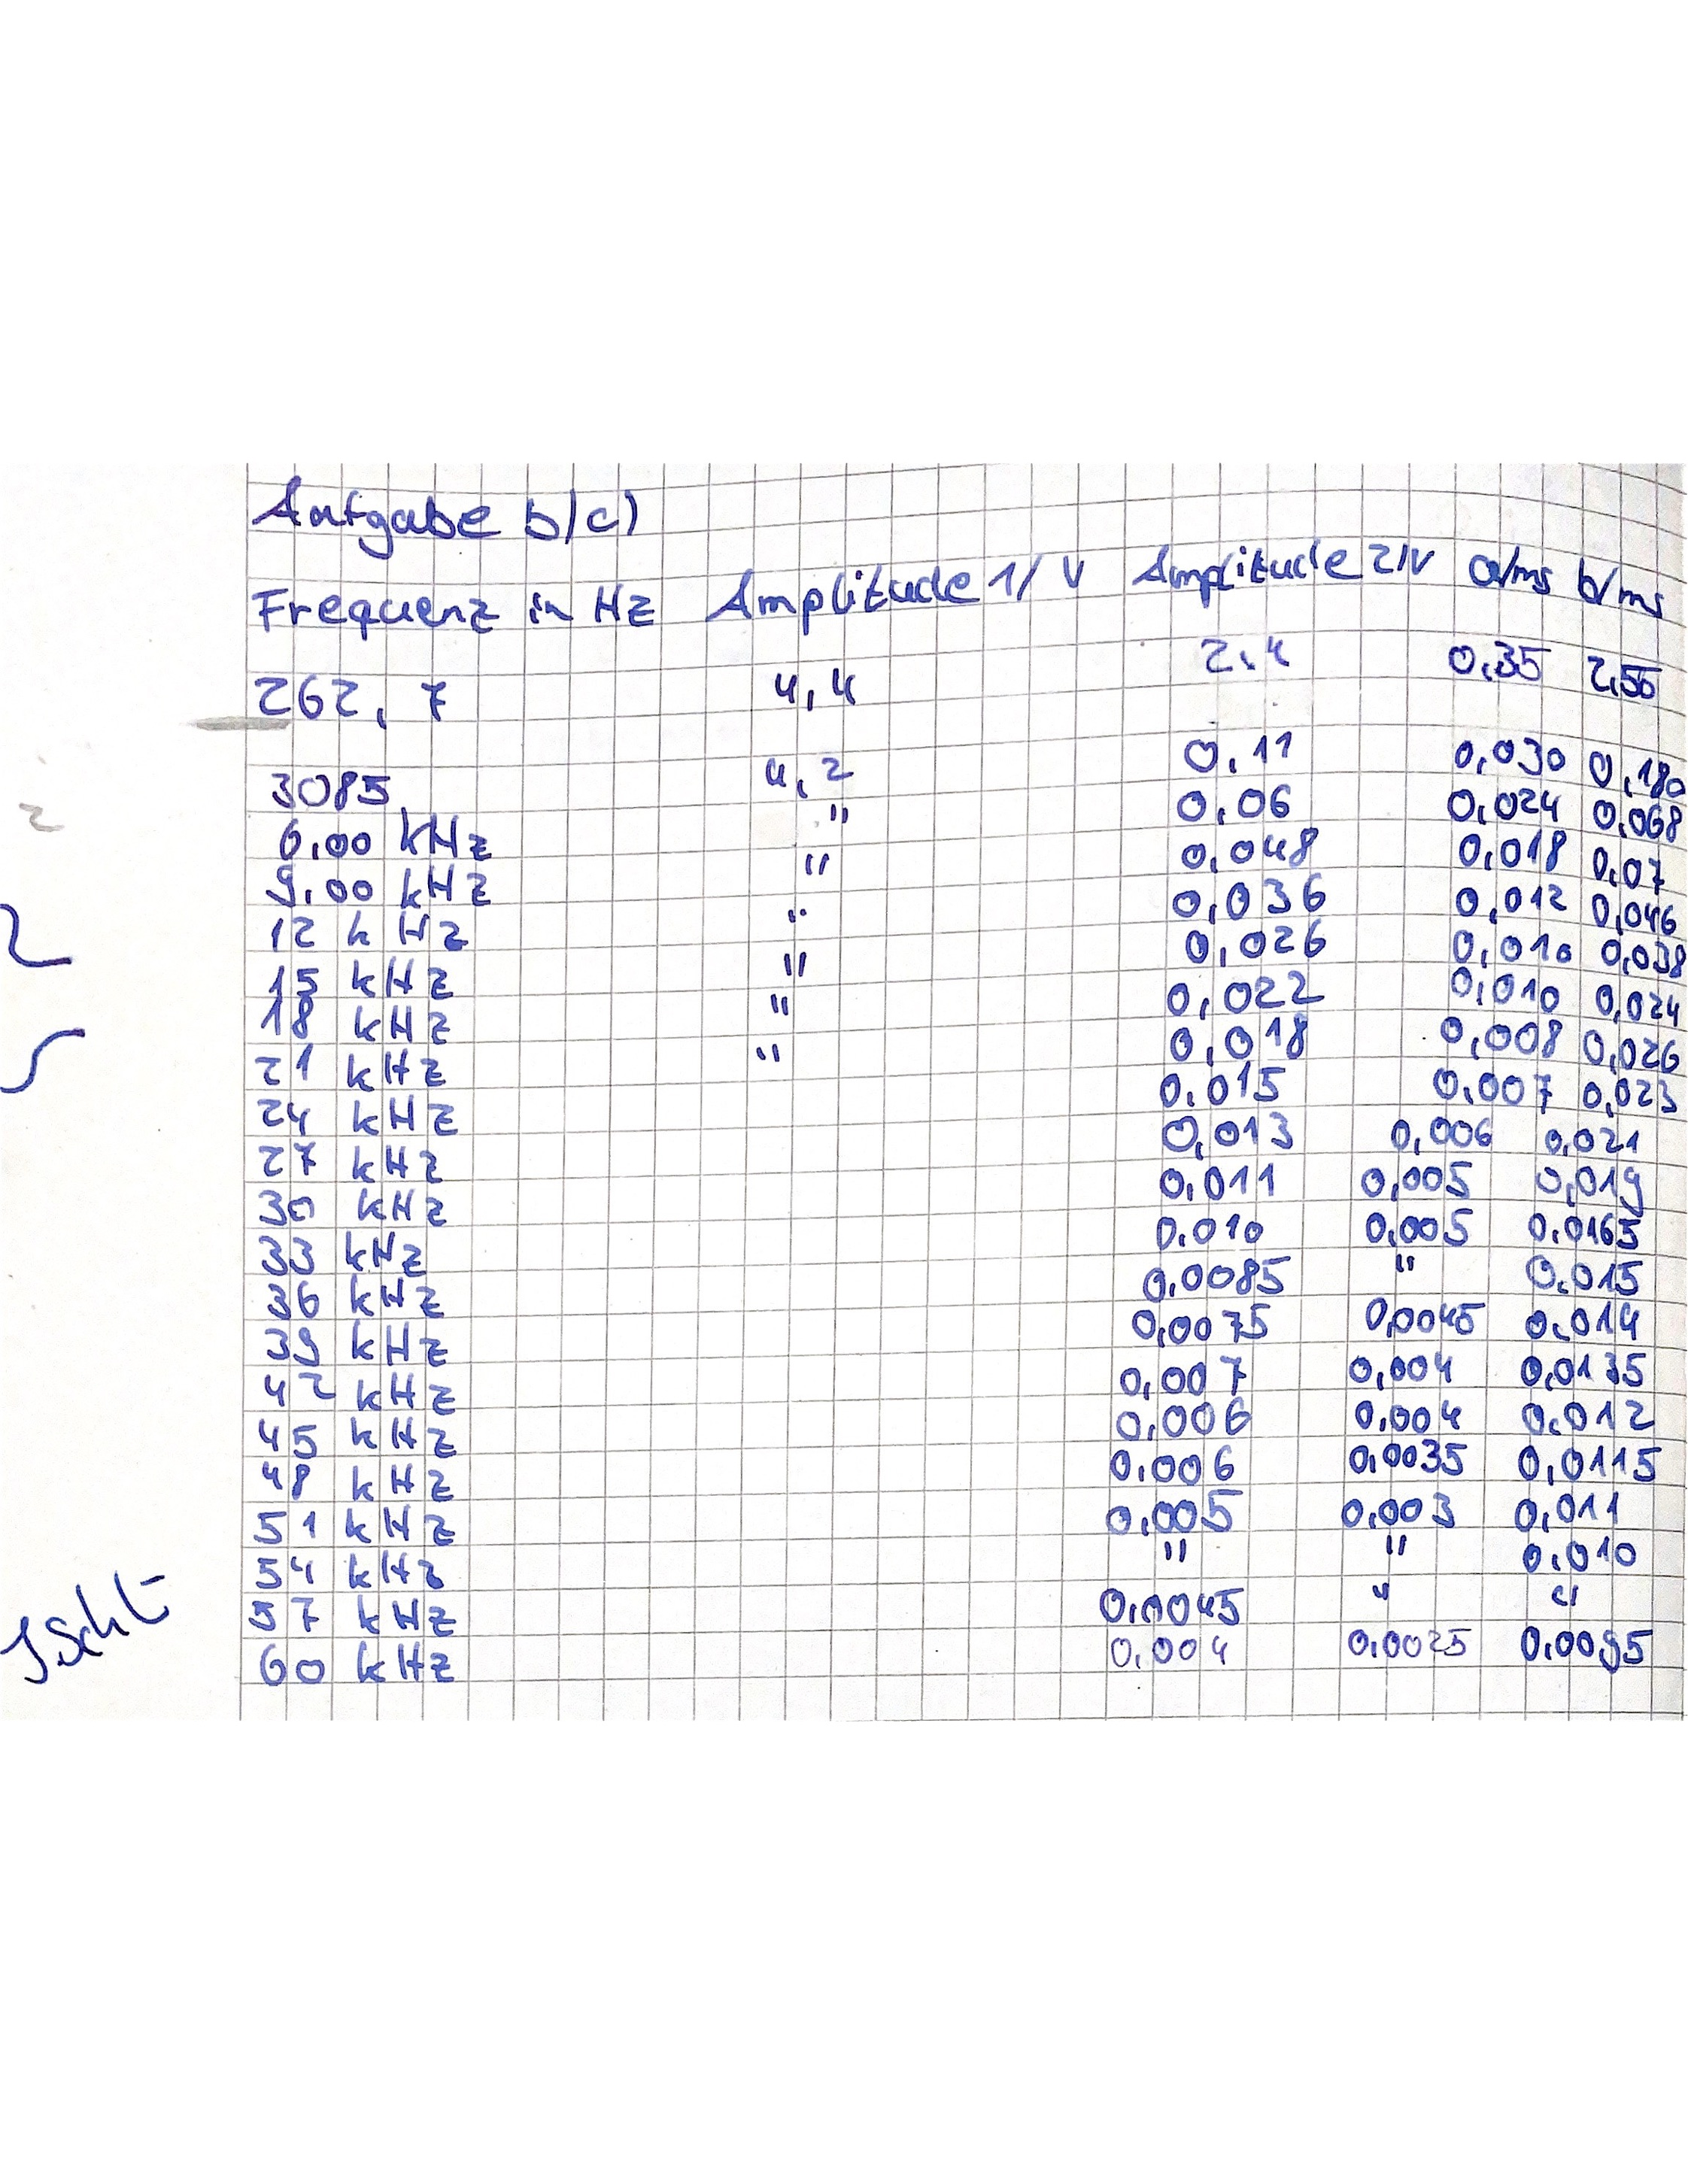
\includegraphics[width=0.75\textwidth]{Dateien/daten2.jpg}
    \caption{Originale Messdaten zu Aufgabenteil b) und c).}
    \label{fig:daten2}
\end{figure}